\chapter{Analyse}

I dette kapitel vil vi gennemgå kravspecifikation til programmet, samt optegne og forklare forskellige modeller.


\section{Kravspecifikation}

Herunder ses en liste over krav til spillet, udformet udfra opgavebeskrivelsen \& det udleverede regelsæt.\footnote{Enkelte krav er hentet fra tidligere CDIO2-rapport af samme gruppe.}

\subsubsection{Alle krav stillet}

\begin{enumerate}
\item Der skal oprettes forskellige typer felter, samt en spilleplade.
\item Hvert felt skal påvirke spillernes pengebeholdning forskelligt, og have en udskrift om hvilket felt han ramte.
\item Spillerne skal kunne lande på et felt, og fortsætte derfra på næste slag.
\item Spillerne skal gå i ring rundt på felterne, på spillepladen, med uret. (man kan ikke gå mod uret)
\item Spillet skal kunne køre på DTU's databar-computere.
\item 2-4 spillere skal kunne spille spillet.
\item Den yngste spiller starter.
\item Hver gang man passerer start, modtager man M2 (penge).
\item Alt efter om der er 2, 3 eller 4 spillere, skal der gives forskellige start-penge.

\item Man skal have mulighed for at vælge hvilket figurkort man vil være. \\Figurkortet vil så have forskellig indflydelse ift. chancekort.

\item Lander en spiller på et ledigt felt, køber spilleren feltet og har nu ejerskab af feltet.
\item Lander en spiller på et ejet felt, betaler denne spiller husleje til den spiller der ejer feltet.
\item Ejer en spiller to egendomme af samme farve, er huslejen det dobbelte af det beløb, der står på feltet.

\item Der skal være tydeligtgjort på spillebrættet hvilke ejede felter, som hører til hvilken spiller.

\item Lander en spiller på et chance felt, skal der vises en beskrivelse af en hændelse, samt en værdi i plus eller minus på spillerens konto.
\item Lander en spiller på et "Gå i fængsel"-felt, flyttes spilleren til "Fængsel". Man får ikke M(penge) ved passage af start.

\item Er en spiller i fængsel, kan man enten betale M1 (penge), eller bruge et chance-kort med løsladelses-mulighed. Mens man er i fængsel tjener man stadig leje.
\item Lander en spiller på "Fængsel", sker der intet.
\item Lander en spiller på "Gratis Parkering", sker der intet.
\item Spillet sluttes, når en spiller ikke har penge nok til at betale husleje, betale en ejendom, eller negativ værdi på et chance-kort.
\item Når spillet er slut, findes den der har flest penge, som så vinder.
\item Har flere spillere samme antal penge, når spillet er slut, tælles alle ejede ejendomsværdi'er, og lægges til pengebeholdningen.

\item (Avanceret) Hvis en spiller ikke har nok penge til at betale husleje eller en afgift fra et chancekort, skal gælden betales med dine ejendomme.
\item (Avanceret) Hvis en spiller skylder penge til en anden spiller, får den spiller dine ejendomme, skylder man banken penge, bliver ejendommene sat til salg igen.
\item (Avanceret) Hvis man skylder penge, og man ikke har nogen penge eller ejendomme, så er man fallit, og spillet slutter.\\
\end{enumerate}

\newpage

\subsubsection{MoSCoW}

MoSCoW, er et værktøj som kan bruges til at prioritere krav.
Herunder ses et eksempel på MoSCoW, og hvad de enkelte kategorier kan indeholde.\footnote{MoSCoW tabellen der vises, er hentet fra tidligere CDIO2-rapport af samme gruppe.} \\\\

\begin{tabular}{lll}
    \textbf{Mo} &   
    "Must have"                 &
    De mest vitale krav, vi ikke kan undgå. \\

    \textbf{S}  &   
    "Should have"               & 
    Vigtige krav, som ikke er vitale. \\

    \textbf{Co} &   
    "Could have"                & 
    The 'nice-to-haves' \\

    \textbf{W}  &   
    "Won’t have (this time)"    & 
    Things that provide little to no value you can give up on \\

\end{tabular}
\\\\

\noindent Vi bruger herunder MoSCoW til at prioriterer vores krav, ved hjælp af MoSCoW.
\begin{center}
    \begin{tabular}{ || p{2.5cm} | p{.4cm} | p{12.4cm} ||}
        \hline
        \hline
         % ------- % * Must have * % ------- %
    &        
    \textbf{1.}
    &
    Der skal oprettes forskellige typer felter, samt en spilleplade. 
    \\

    \cline{2-3}
    &
    \textbf{2.}
    & 
    Hvert felt skal påvirke spillernes pengebeholdning forskelligt, og have en udskrift om hvilket felt han ramte. 
    \\
    
    \cline{2-3}
    &
    \textbf{3.}
    &
    Spillerne skal kunne lande på et felt, og fortsætte derfra på næste slag.
    \\

    \cline{2-3}
    &
    \textbf{4.}
    &
    Spillerne skal gå i ring rundt på felterne, på spillepladen, med uret. (man kan ikke gå mod uret)
    \\

    \cline{2-3}
    &
    \textbf{5.} 
    &
    Spillet skal kunne køre på DTU’s databar-computere.
    \\
    
    \cline{2-3}
    \textbf{Must have}
    &
    \textbf{6.}
    &
    2-4 spillere skal kunne spille spillet.
    \\
    
    \cline{2-3}
    &
    \textbf{11.}
    &
    Lander en spiller på et ledigt felt, køber spilleren feltet og 
    har nu ejerskab af feltet.
    \\

    \cline{2-3}
    &
    \textbf{12.}
    &
    Lander en spiller på et ejet felt, betaler denne spiller husleje til den spiller der ejer feltet.
    \\

    \cline{2-3}
    &
    \textbf{20.}
    &
    Spillet sluttes, når en spiller ikke har penge nok til at betale husleje, betale en ejendom, eller negativ værdi på et chance-kort.
    \\

    \cline{2-3}
    &
    \textbf{21.}
    &
    Når spillet er slut, findes den der har flest penge, som så vinder.
    \\
    
    \hline
    \hline
     % ------- % * Should have * % ------- %
     &
     \textbf{14.}
     &
     Der skal være tydeligtgjort på spillebrættet hvilke ejede felter, som hører til hvilken spiller.
     \\

     \cline{2-3}
     &
     \textbf{15.}
     &
     Lander en spiller på et chance felt, skal der vises en beskrivelse af en hændelse, samt en værdi i plus eller minus på spillerens konto.
     \\

     \cline{2-3}
     &
     \textbf{16.}
     &
     Lander en spiller på et "Gå i fængsel"-felt, flyttes spilleren til "Fængsel". Man får ikke M(penge) ved passage af start.
     \\
    
     \cline{2-3}
     \textbf{Should have}
     &
     \textbf{18.}
     &
     Lander en spiller på "Fængsel", sker der intet. \\
    
     \cline{2-3}
     &
     \textbf{19.}
     &
     Lander en spiller på "Gratis Parkering", sker der intet. 
     \\

     \hline
     \hline
     % ------- % * Could have * % ------- %
     &
     \textbf{7.}
     &
     Den yngste spiller starter.
     \\

     \cline{2-3}
     &
     \textbf{8.}
     &
     Hver gang man passerer start, modtager man M2 (penge).
     \\
     
     \cline{2-3}
     \textbf{Could have}
     &
     \textbf{9.}
     &
     Alt efter om der er 2, 3 eller 4 spillere, skal der gives forskellige start-penge.
     \\

     \cline{2-3}
     &
     \textbf{10.}
     &
     Man skal have mulighed for at vælge hvilket figurkort man vil være.
     Figurkortet vil så have forskellig indflydelse ift. chancekort. 
     \\

     \cline{2-3}
     &
     \textbf{13.}
     &
     Ejer en spiller to egendomme af samme farve, er huslejen det dobbelte af det beløb, der står på feltet.
     \\

     \cline{2-3}
     &
     \textbf{17.}
     &
     Er en spiller i fængsel, kan man enten betale M1 (penge), eller bruge et chance-kort med løsladelses-mulighed. Mens man er i fængsel tjener man stadig leje. 
     \\

    \hline
    \hline
    % ------- % * Won't have * % ------- %
    &
    \textbf{22.}
    &
    Har flere spillere samme antal penge, når spillet er slut, tælles alle ejede ejendomsværdi'er, og lægges til pengebeholdningen. \\

    \cline{2-3}
    \textbf{Won't have}
    &
    \textbf{23.}
    &
    (Avanceret) Hvis en spiller ikke har nok penge til at betale husleje eller en afgift fra et chancekort, skal gælden betales med dine ejendomme.
    \\

    \cline{2-3}
    &
    \textbf{24.}
    &
    (Avanceret) Hvis en spiller skylder penge til en anden spiller, får den spiller dine ejendomme, skylder man banken penge, bliver ejendommene sat til salg igen.
    \\

    \cline{2-3}
    &
    \textbf{25.}
    &
    (Avanceret) Hvis man skylder penge, og man ikke har nogen penge eller ejendomme, så er man fallit, og spillet slutter. \\
    \hline
    \hline
    \end{tabular}
\end{center}

\subsubsection{FURPS+}

FURPS+ er en metode til at kategorisere / klassificere krav. \\
Vi har i denne opgave brugt FURPS+ metoden til at kategorisere de krav, som er prioriteret i MoSCoW analysen.
Vi har ikke valgt at medtage alle FURPS+ punkterne, men medbragt dem der giver mening for opgaven. \\
Herunder ses et eksempel på FURPS+, og hvad de enkelte kategorier kan indeholde.\footnote{FURPS+ tabellen der vises, er hentet fra tidligere CDIO2-rapport af samme gruppe.}

\begin{figure*}[ht]{
    \centering
\begin{tabular}{|c | p{0,05cm} p{2,8cm} |p{10,5cm}|}
       \hline
       \textbf{F}   &   Functionality   &&
       Egenskaber, ydeevne, sikkerhed                   \\
       \hline

       \textbf{U}   &   Usability       &&
       Menneskelige faktorer, hjælp, dokumentation      \\
       \hline

       \textbf{R}   &   Reliability     &&
       Fejlfrekvens, fejlretning, forudsigelighed       \\
       \hline

       \textbf{P}   &   Performance     &&
       Svartider, nøjagtighed, ydeevne, ressourceforbrug                                                      \\
       \hline

       \textbf{S}   &   Supportability  &&
       Anvendelighed, tilpasningsevne, vedligeholdbarhed                                                      \\
       \hline

       \textbf{+}   &                   &&              \\

       &&   Implementation: &   Ressourcebegrænsninger, sprog og værktøjer, hardware                     \\

       &&   Interface:      &   Begrænsninger forårsaget af kommunikation med eksterne systemer              \\

       &&   Operations:     &   Systemstyring i dets operationelle ramme                              \\

       &&   Packaging:      &   F.eks. en fysisk boks   \\

       &&    Legal:         &   F.eks. licenser       \\
       \hline
\end{tabular}}
\end{figure*}

\pagebreak

\noindent Vi her herunder en oversigt over krav til opgaven, \\ kategoriseret ved hjælp af FURPS+. Der er ikke medtaget de krav der er i "Won't have" kategorien i MoSCoW-analysen.
\\\\\textbf{Functionality:}\\
    \textbf{8.} Hver gang man passerer start, modtager man M2 (penge). 
    \\
    \textbf{9.} Alt efter om der er 2, 3 eller 4 spillere, skal der gives forskellige start-penge. 
    \\
    \textbf{11.} Lander en spiller på et ledigt felt, køber spilleren feltet og har nu ejerskab af feltet. 
    \\
    \textbf{12.} Lander en spiller på et ejet felt, betaler denne spiller husleje til den spiller der ejer feltet. 
    \\
    \textbf{13.} Ejer en spiller to egendomme af samme farve, er huslejen det dobbelte af det beløb, der står på feltet. 
    \\
    \textbf{15.} Lander en spiller på et chance felt, skal der vises en beskrivelse af en hændelse, samt en værdi i plus eller minus på spillerens konto. 
    \\
    \textbf{16.}
    Lander en spiller på et "Gå i fængsel"-felt, flyttes spilleren til "Fængsel". Man får ikke M(penge) ved passage af start. 
    \\
    \textbf{17.}
    Er en spiller i fængsel, kan man enten betale M1 (penge), eller bruge et chance-kort med løsladelses-mulighed. Mens man er i fængsel tjener man stadig leje. 
    \\
    \textbf{18.} Lander en spiller på "Fængsel", sker der intet. 
    \\
    \textbf{19.} Lander en spiller på "Gratis Parkering", sker der intet. 
    \\
    \textbf{20.} Spillet sluttes, når en spiller ikke har penge nok til at betale husleje, betale en ejendom, eller negativ værdi på et chance-kort. \\
    \textbf{21.} Når spillet er slut, findes den der har flest penge, som så vinder. Har flere spillere samme antal penge, tælles alle ejede ejendomsværdi’er, og lægges til pengebeholdningen.
\\\\\textbf{Usability:}\\
    \textbf{6.} 2-4 spillere skal kunne spille spillet.
\\\\\textbf{(+) - Interface:}\\
    \textbf{1.} Der skal oprettes forskellige typer felter, samt en spilleplade. 
    \\
    \textbf{14.} Der skal være tydeligtgjort på spillebrættet hvilke ejede felter, som hører til hvilken spiller. 
    \\
    \textbf{2.} Hvert felt skal påvirke spillernes pengebeholdning forskelligt, og have en udskrift om hvilket felt han ramte. 
    \\
    \textbf{3.} Spillerne skal kunne lande på et felt, og fortsætte derfra på næste slag. 
    \\
    \textbf{4.} Spillerne skal gå i ring rundt på felterne, på spillepladen, med uret. (man kan ikke gå mod uret) 
    \\
    \textbf{7.} Den yngste spiller starter. 
    \\
    \textbf{10.} Man skal have mulighed for at vælge hvilket figurkort man vil være.
    
    Figurkortet vil så have forskellig indflydelse ift. chancekort.
\\\\\textbf{(+) - Operations:}\\
    \textbf{5.} Spillet skal kunne køre på DTU’s databar-computere. 
    \\

    \pagebreak
\subsubsection{Implementerede krav}

Herunder ses de krav, der ved hjælp af MoSCoW er blevet udvalgt til at blive implementeret i programmet. 
\\

\begin{tabular}{| l |p{13cm}|}

    \hline
    \textbf{1.} 
    &
    Der skal oprettes forskellige typer felter, samt en spilleplade. 
    \\
    
    \hline
    \textbf{2.} 
    &
    Hvert felt skal påvirke spillernes pengebeholdning forskelligt, og have en udskrift om hvilket felt han ramte. 
    \\
    
    \hline
    \textbf{3.} 
    &
    Spillerne skal kunne lande på et felt, og fortsætte derfra på næste slag. 
    \\
    
    \hline
    \textbf{4.} 
    &
    Spillerne skal gå i ring rundt på felterne, på spillepladen, med uret. 

    (man kan ikke gå mod uret) 
    \\
    
    \hline
    \textbf{5.} 
    &
    Spillet skal kunne køre på DTU’s databar-computere. 
    \\
    
    \hline
    \textbf{6.} 
    &
    2-4 spillere skal kunne spille spillet. 
    \\

    \hline
    \textbf{7.} 
    &
    Den yngste spiller starter. 
    \\
      
    \hline
    \textbf{8.}
    &
    Hver gang man passerer start, modtager man M2 (penge). 
    \\
      
    \hline
    \textbf{9.}
    &
    Alt efter om der er 2, 3 eller 4 spillere, skal der gives forskellige start-penge. 
    \\

    \hline
    \textbf{10.}
    &
    Man skal have mulighed for at vælge hvilket figurkort man vil være.
    
    Figurkortet vil så have forskellig indflydelse ift. chancekort. 
    \\
      
    \hline
    \textbf{11.}
    &
    Lander en spiller på et ledigt felt, køber spilleren feltet og har nu ejerskab af feltet. 
    \\
      
    \hline
    \textbf{12.}
    &
    Lander en spiller på et ejet felt, betaler denne spiller husleje til den spiller der ejer feltet. 
    \\
      
    \hline
    \textbf{13.}
    &
    Ejer en spiller to egendomme af samme farve, er huslejen det dobbelte af det beløb, der står på feltet. 
    \\
    
    \hline
    \textbf{14.} 
    &
    Der skal være tydeligtgjort på spillebrættet hvilke ejede felter, som hører til hvilken spiller. 
    \\
      
    \hline
    \textbf{15.}
    &
    Lander en spiller på et chance felt, skal der vises en beskrivelse af en hændelse, samt en værdi i plus eller minus på spillerens konto. 
    \\

    \hline
    \textbf{16.}
    &
    Lander en spiller på et "Gå i fængsel"-felt, flyttes spilleren til "Fængsel". Man får ikke M(penge) ved passage af start. 
    \\
      
    \hline
    \textbf{17.}
    &
    Er en spiller i fængsel, kan man enten betale M1 (penge), eller bruge et chance-kort med løsladelses-mulighed. Mens man er i fængsel tjener man stadig leje. 
    \\
      
    \hline
    \textbf{18.}
    &
    Lander en spiller på "Fængsel", sker der intet. 
    \\
      
    \hline
    \textbf{19.}
    &
    Lander en spiller på "Gratis Parkering", sker der intet. 
    \\
      
    \hline
    \textbf{20.}
    &
    Spillet sluttes, når en spiller ikke har penge nok til at betale husleje, betale en ejendom, eller negativ værdi på et chance-kort. 
    \\
      
    \hline
    \textbf{21.}
    &
    Når spillet er slut, findes den der har flest penge, som så vinder. 
    
    Har flere spillere samme antal penge, tælles alle ejede ejendomsværdi’er, og lægges til pengebeholdningen. 
    \\
      
    \hline
\end{tabular}

\pagebreak

\section{Interessentanalyse}

    \begin{tabular}{ | l | p{13cm} |}
      
      \hline
    \textbf{Interresent} & \textbf{Interesse / Mål} \\ \hline
    Spillere & Kunne styre et system, der styrer et spil mellem 2-4 personer, 
    hvor i der kastes en terning, og man ser resultatet af dette slag med det samme, herefter skal facevaluen af dette slag fortælle, hvilket felt spilleren landte på, derudover skal den kunne fortælle om feltet er ejet, eller om det er frit til at købe, således at man enten skal betale til en spiller, eller har mulighed for at købe grunden.
    \\ 
    \hline
      
    \hline
    \end{tabular}

\section{Use case diagram}
Use cases bliver lavet for at skabe overblik over det kommende program.
Ligeledes har vi valgt at inddrage et use case-diagram for at illustrere, hvordan det ser ud for vores program.
Use case-diagrammet er meget beskedent, idet der kun er én aktør, nemlig spilleren, som kun kan gøre én ting, nemlig at spille spillet.
\begin{figure}[H]
    \begin{center}
        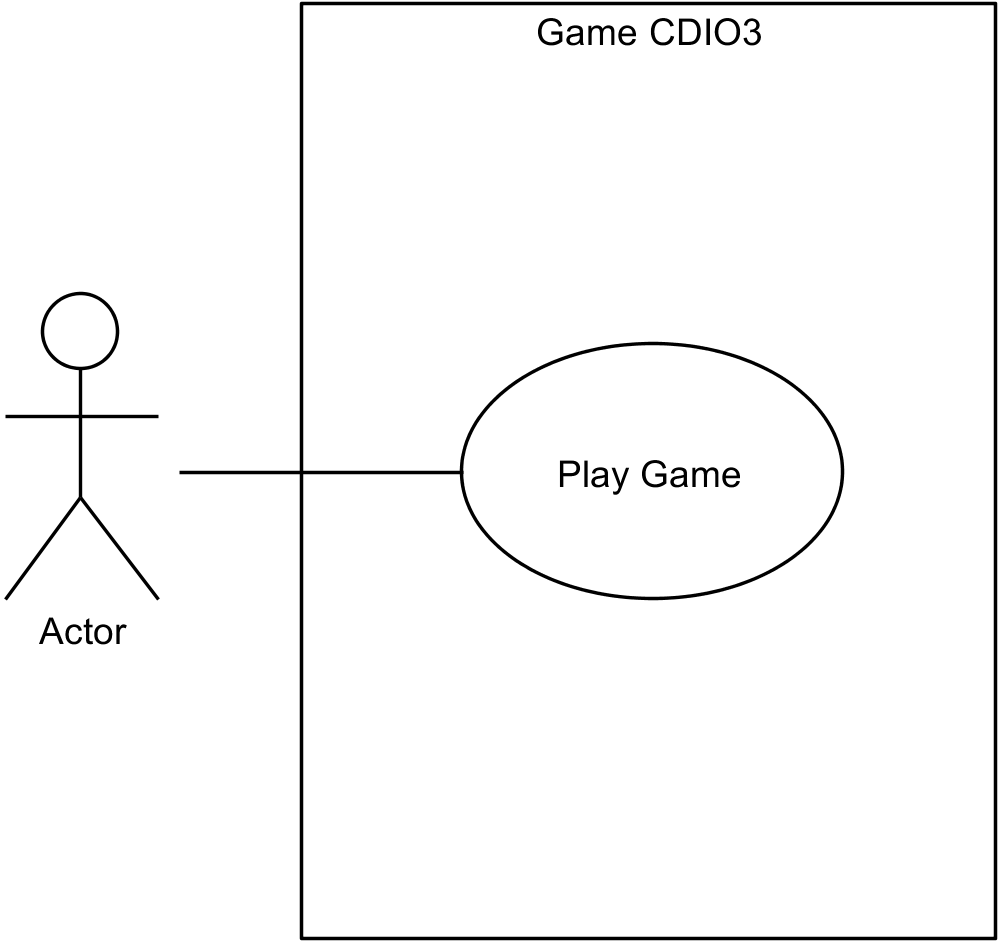
\includegraphics[width=10cm]{graphics/usecases/UseCase1.png}
        \caption{Use case diagram}
        \label{fig:use_case_diagram}
    \end{center}
\end{figure}

\pagebreak

\section{Use case}
\subsubsection{Brief}
Spillet starter med en dropdown menu hvorpå der angives antallet af deltagende spillerer.
Efterfølgende indtastes navn på spillerene og efterfulgt af endnu en dropdown menu med det formål at vælge den yngste spiller.
Før spillets start tildeles de hver en pengebeholdning.
Den yngste spiller starter og kaster derved med terningen.
Terningen øje eller faceValue tages og bruges som udgangspunkt til bergening af hvor mange felter spilleren skal flytte sig.
På GUI'en vises feltets oplysninger, samt hvorvidt det er ejet eller ej.
Der slås igen med terningen, spilleren lander på et felt, og et bestemt scenarie tages i brug, afhængig af felt oplysningerne, hvor så samme procedure følger indtil en spiller ærklæres bankerot.
Der tælles point på spillerne, og spilleren med den største pengebeholdning vinder spillet.\\

\subsubsection{Fully dressed}
Følgende er en beskrivelse af use casen 'playGame' i en fully dressed udgave.

\begin{table}[H]
    \begin{center}
        \begin{tabular}{ | p{15cm} |}
            \hline
            \textbf{Use case:} PlayGame \\ \hline
            \textbf{ID:} UC1 \\ \hline
            \textbf{Brief description} Spillere skal kunne spille spillet, altså playGame og slå med en terning.     \\ \hline
            \textbf{Primary actors:} Spillere \\ \hline
            \textbf{Secondary actors:} Ingen. \\ \hline
            \textbf{Preconditions:}      \\ \hline
            \textbf{Main flow:}
            \begin{enumerate}
                \item \textbf{Spillet startes, antal spillere vælges (minimum 2 og maksimum 4 spillere) samt indtaster deres navn. Den yngste spiller specificeres, og er den første der slår med terningen.}
                \item \textbf{Spillet flytter spilleren afhængig af faceValue fra terningen.}
                \item \textbf{Feltets oplysninger udskrives til spilleren via GUI.}
                \item \textbf{Ny runde finder sted, og næste spiller kaster med terningen.}
                \item \textbf{Spillet giver nye ture indtil at en af spillerens pengebeholdning går i minus eller ikke har råd til købe/betaling af ejendom.}
                \item \textbf{Går en spillers pengebeholdning i minus, erklæres hermed spilleren bankerot, og spillet slutter}
            \end{enumerate} \\ \hline
            \textbf{Postconditions:} Ingen.\\ \hline
            \textbf{Alternative flow:}
            \begin{enumerate}
                \item \textbf{Spiller lander på ikke ejet felt}
                \begin{enumerate}
                    \item {Spiller køber felt.}
                    \item {Spiller bliver tildelt felt.}
                \end{enumerate}
                \item \textbf{Spiller lander på ejet felt}
                \begin{enumerate}
                    \item {Spiller betaler ejeren af felt. Har ejeren mere end et felt, betales dobbelt beløb.}
                    \item {Ejer modtager beløb.}                    
                \end{enumerate}
                \item \textbf{Spiller passerer start felt}
                \begin{enumerate}
                    \item {Spiller får adderet 2M i sin pengebeholdning.}
                \end{enumerate}
                \item \textbf{Spiller lander på fængsel felt}
                \begin{enumerate}
                    \item {Spiller flyttes til fængsel feltet.}
                    \item {Spiller modtager ikke 2M ved passering af start feltet.}
                    \item {Spiller betaler 1M efter løsladelse fra fængsel, eller ved brug af 'Du løslades uden omkostninger' kortet.}
                \end{enumerate}
            \end{enumerate} \\ \hline
            \hline
        \end{tabular}
        \caption{Use case 1}
        \label{usecase:1}
    \end{center}
\end{table}

\newpage
\section{Risicianalyse}
For at skabe et overblik over de risici, som kan forekomme i udviklingsprocessen, oprettes der en risicitabel, som fortæller om risicien, dens påvirkning (skala 1-10, hvor 1 er mindst, 10 er højest) samt påvirkningsgrad (samma skala). \\ \\
Der er udelukkende blevet oprettet en risicitabel over udviklingsprocessen og altså ikke de forskellige use cases, hvilket man i den agile udviklingsmetode, Unified Process, normalvis ville gøre brug af, da man ønsker at lave de højstprioriterede use cases indledningsvis.

\begin{enumerate}
    \item \textbf{Problemer med GUI.} \\
    Påvirkning = 10\\ Sandsynlighed = 8.\\
    Det er klart, at spillet skal se godt ud og ikke skal køre i kommandoprompt/terminal.
    Vi arbejdede med GUI i CDIO2, men da der er kommet ny GUI, kan der også opstå nye problemer, derfor er det vigtigt at tage højde for dette i god tid og læse op på dokumentationen, om hvordan man bruger GUI'en.
    \item \textbf{Overtrædelse af deadline.} \\
    Påvirkning = 3\\ Sandsynlighed = 10.\\
    Vi bruger Asana til at give hinanden lektier for og holde styr på, hvad vi mangler i projektet.
    Vi har strategisk valgt at sætte os til at lave tingene i god tid, således vi kan tage højde for eventuelle problemer, og det er derfor ikke et stort problem, hvis deadline bliver overtrædt (i begyndelsen).
    \item \textbf{Problemer med design af kode.} \\
    Påvirkning = 7\\ Sandsynlighed = 8.\\
    Ligesom i de foregående projekter, kan man hurtigt komme til at følge en vandfaldsmodel, idet man tegner en masse diagrammer, men så hænger det ikke sammen med, hvordan spillet rent faktisk kommer til at fungere.
    Vi prøver til vores bedste evner at designe og kode parallelt.
    
\end{enumerate}

De ovenstående situationer er blevet skrevet op for at gøre os opmærksomme på de potentielle vanskeligheder i udviklingsprocessen.

\section{Domænemodel}

\begin{figure}[H]
    \begin{center}
        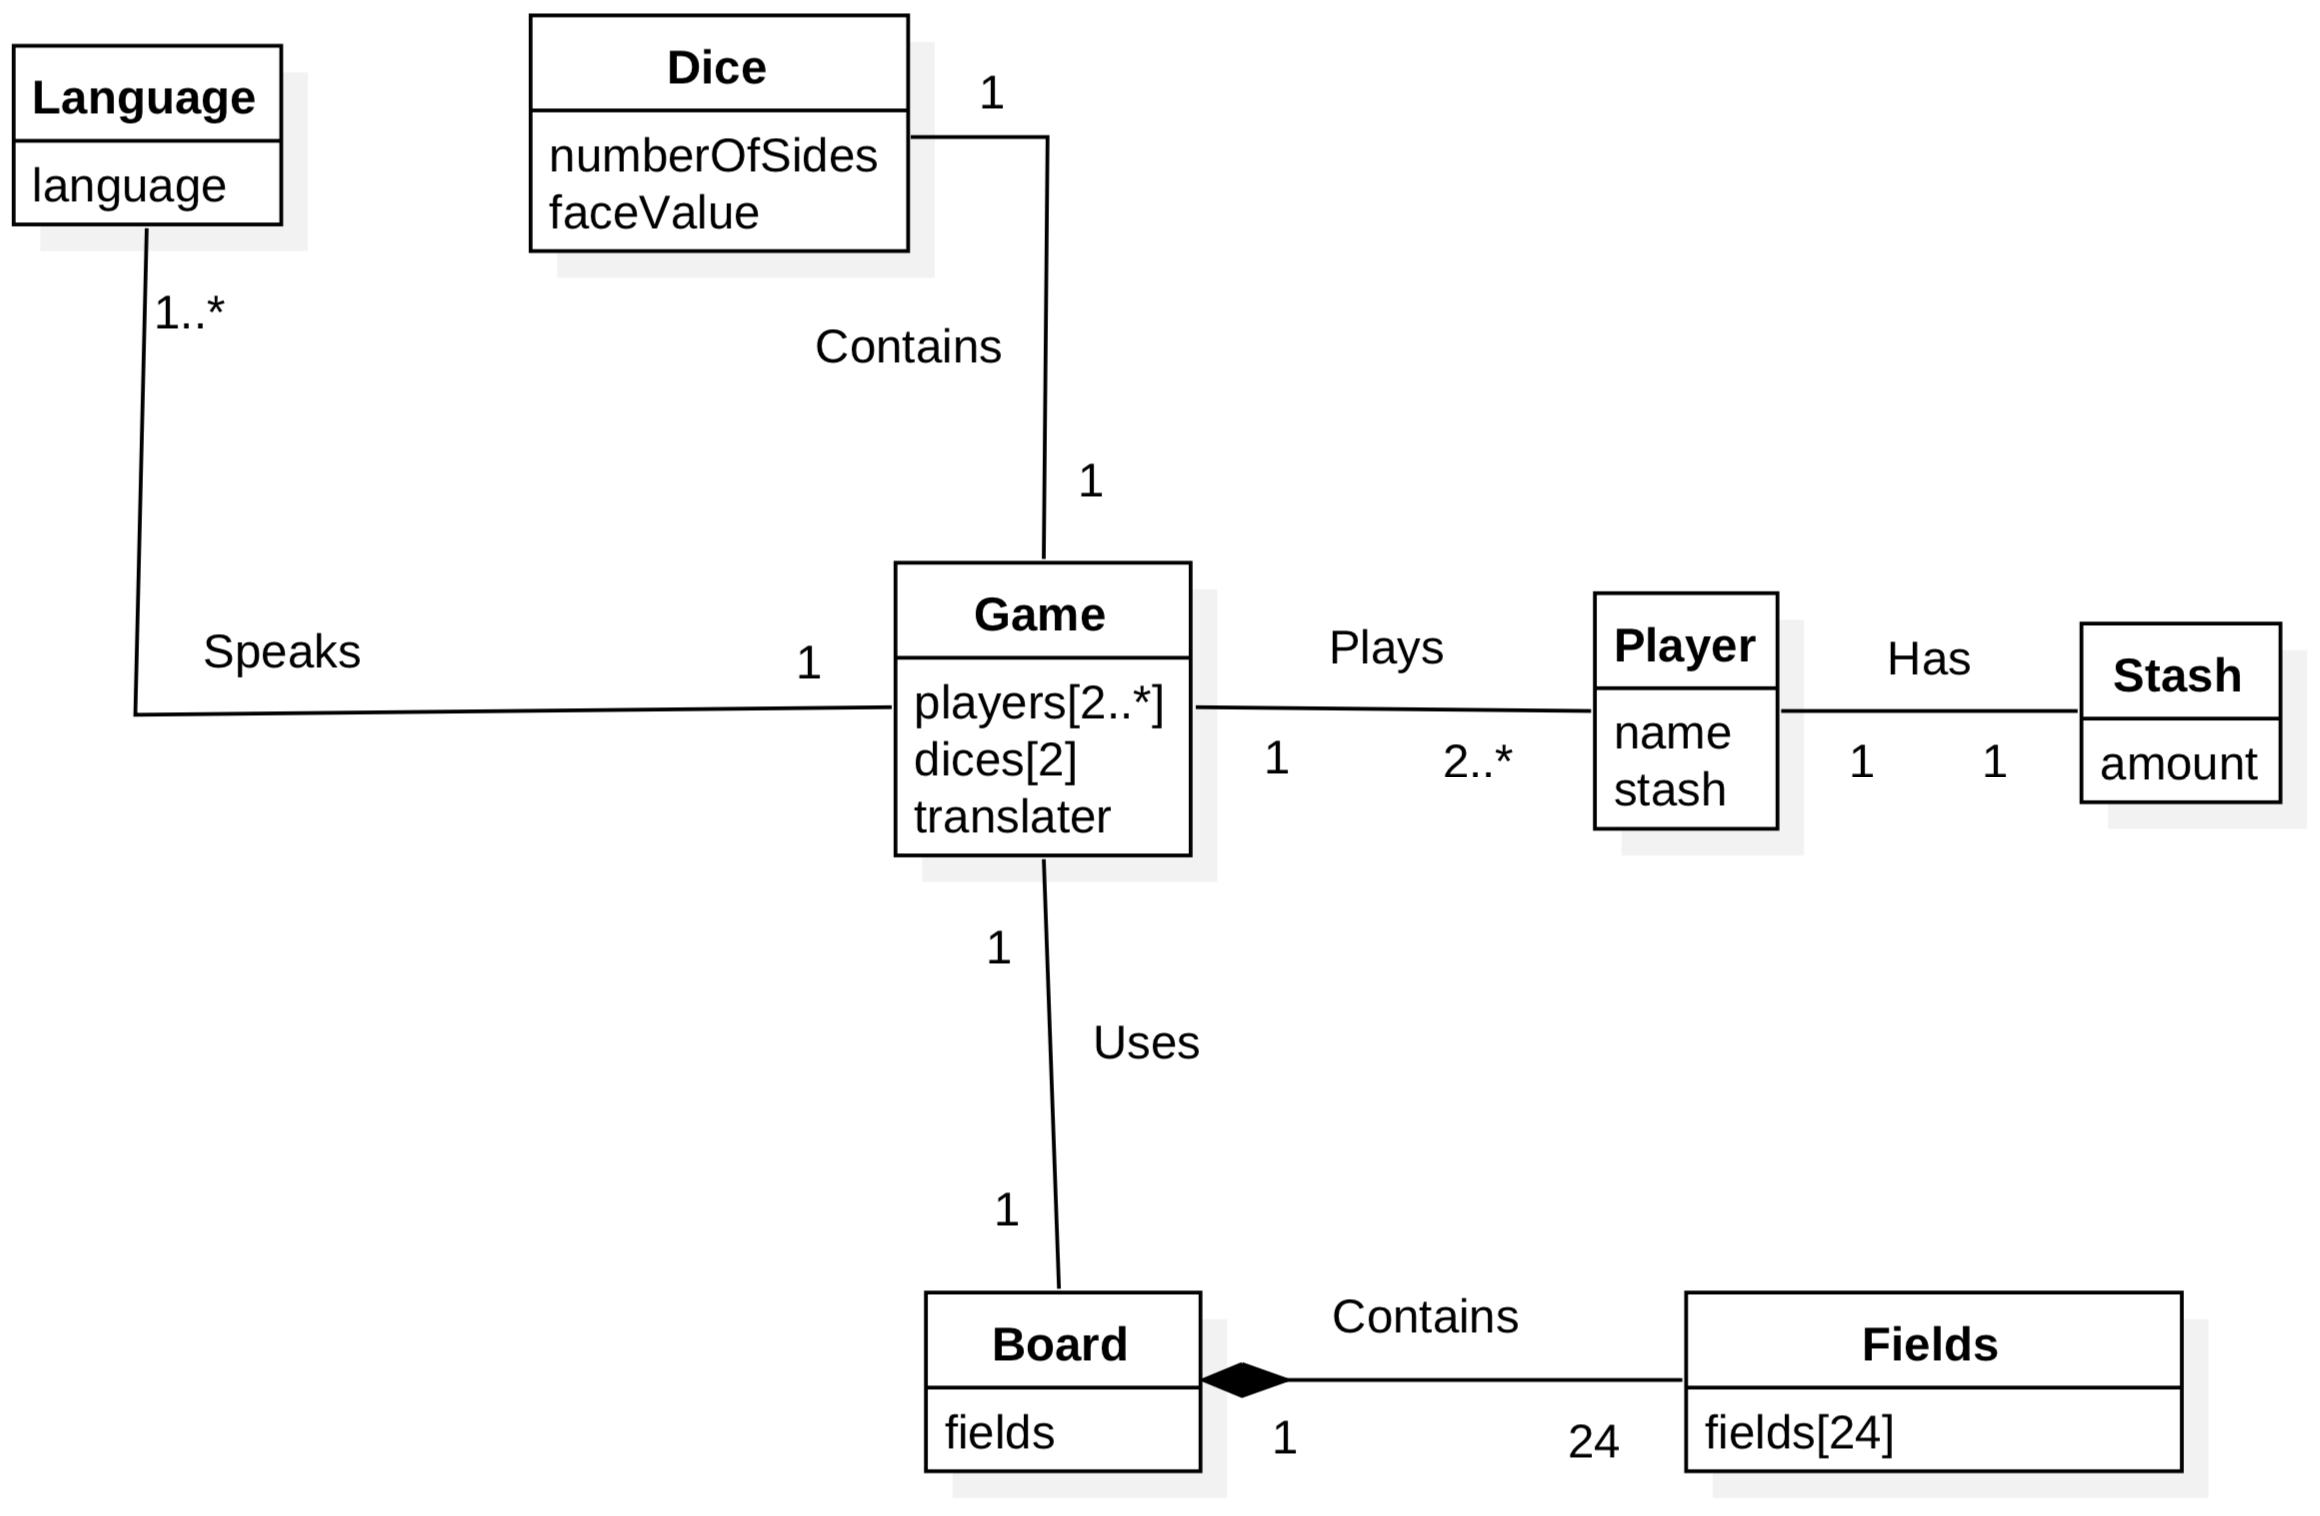
\includegraphics[width=\columnwidth]{graphics/domain/Domainmodel.png}
        \caption{Domænemodel}
        \label{fig:use_case_diagram}
    \end{center}
\end{figure}